\chapter{Specialized Architectures}
Le architetture specializzate si rivolgono principalmente a problemi di ottimizzazione di storage e networking, e hanno lo scopo di massimizzare le prestazioni negli scenari dove è più diffile richiederle. Infatti storage e network, che sono punti chiave dei sistemi informativi, possono essere collegati rispettivamente agli obiettivi di prestazioni e ridondanza.

L'approccio a queste architetture è particolarmente pragmatico, cercando di eliminare quei livelli di astrazione spesso introdotti per facilitare l'organizzazione ma che degradano le prestazioni. La domanda è semplice: dopo quanto tempo dalla lettura di un'istruzione questa viene eseguita effettivamente dall'hardware? La risposta non è altrettanto semplice, basti pensare a tutti i livelli di astrazione posti dalle macchine virtuali, dagli hypervisor e da altre componenti non strettamente necessarie.

A differenza del libro, queste architetture sono riorganizzate in base al loro obiettivo: architetture legate allo storage e architetture legate alla rete.

\section{Storage related architectures}
\subsection{Direct I/O Access}
L'accesso alle schede di I/O fisiche (quindi i server fisici) spesso avviene da parte dei server virtuali tramite un livello composto da hypervisor, chiamato livello di virtualizzazione I/O. Questa architettura permette l'accesso diretto alle schede di I/O fisiche da parte dei virtual server senza passare per questo livello intermedio.

\begin{figure}[htb!]
    \centering
    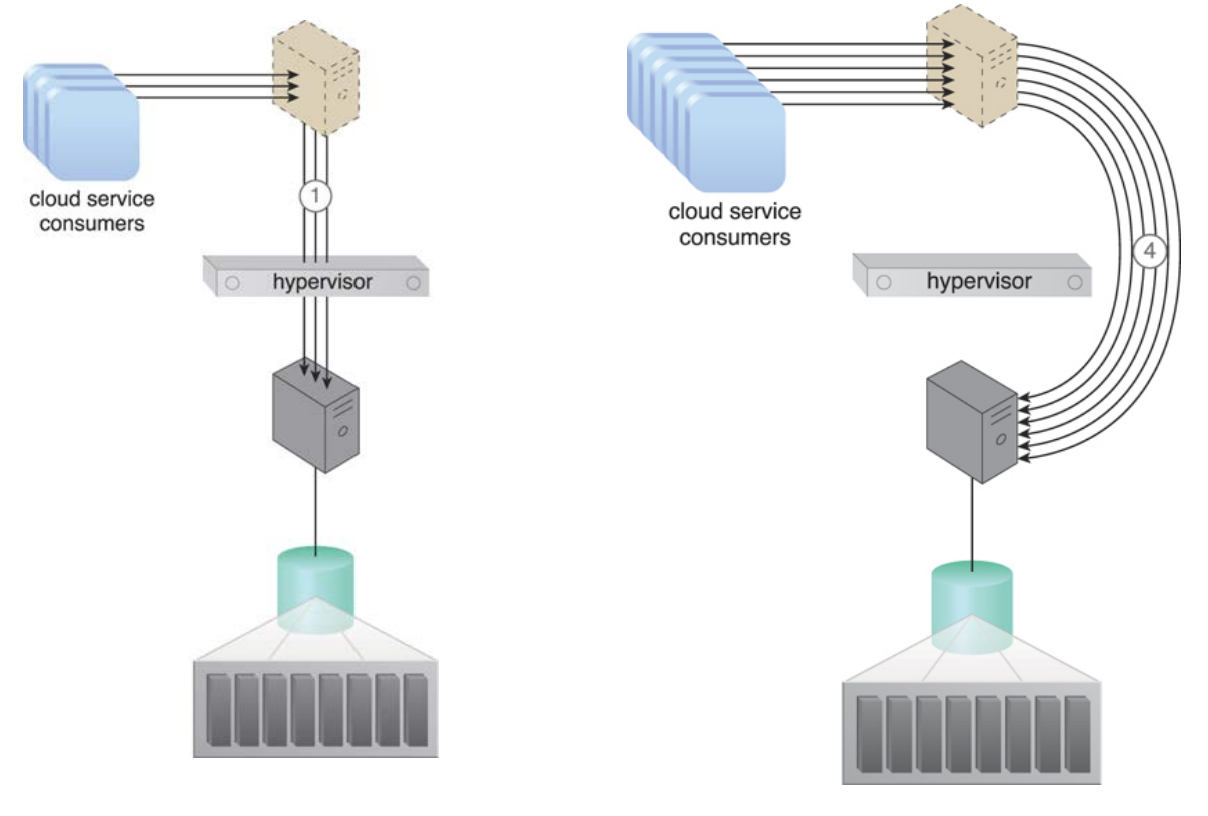
\includegraphics[width=10cm]{./Images/cap13/13.1.png}
\end{figure}

Di norma l'accesso viene fatto dalla macchina virtuale tramite un hypervisor che sta su un server fisico, il quale ha accesso al disco. L'aumento di richieste da parte dei cloud service consumer può causare problemi di prestazioni e portare a un bottle neck per l'hypervisor. N.B. Qui si parla di un collo di bottiglia per l'accesso allo storage, non per la computazione. La soluzione sta nel permettere al server virtuale di bypassare l'hypervisor e connettersi così al database attraverso un link fisico che permette di accedere direttamente allo storage.

I meccanismi utilizzati sono:
\begin{itemize}
    \item Virtual server
    \item Hypervisor
    \item Cloud Usage Monitor, che raccoglie dati sugli accessi diretti all'I/O. A causa dell'accesso diretto bisogna calcolare il costo specifico perché non è presente un load balancer.
    \item Logical Network Perimeter, in quanto le schede I/O fisiche sono accessibili dall'interno del perimetro.
    \item Pay-Per-Use Monitor, come detto prima.
    \item Resource Replication, per rimpiazzare le schede di I/O virtuali con schede I/O fisiche.
\end{itemize}

\subsection{Direct LUN Access}
Anche quest'architettura permette di bypassare la virtualizzazione per migliorare le prestazioni dello storage. Tipicamente le LUN riguardanti lo storage sono mappate tramite un \textbf{Host Bus Adapter} (HBA) sugli hypervisor, mentre lo spazio di archivazione viene emulato sui virtual server. Tuttavia a volte può essere necessario accedere direttamente allo storage in quanto l'emulazione non è sufficiente per il cluster quando questo deve hostare la LUN.

Viene fornito quindi un accesso tramite questo HBA, che permette di accedere anche ai volumi del disco che sono utilizzati nel cluster. In questo modo la connessione fisica ai virtual server da parte delle LUN viene attivata dagli stessi host fisici. Le LUN quindi sono create e configurate sul cloud storage device per accedere anche a device fisici.

\begin{figure}[htb!]
    \centering
    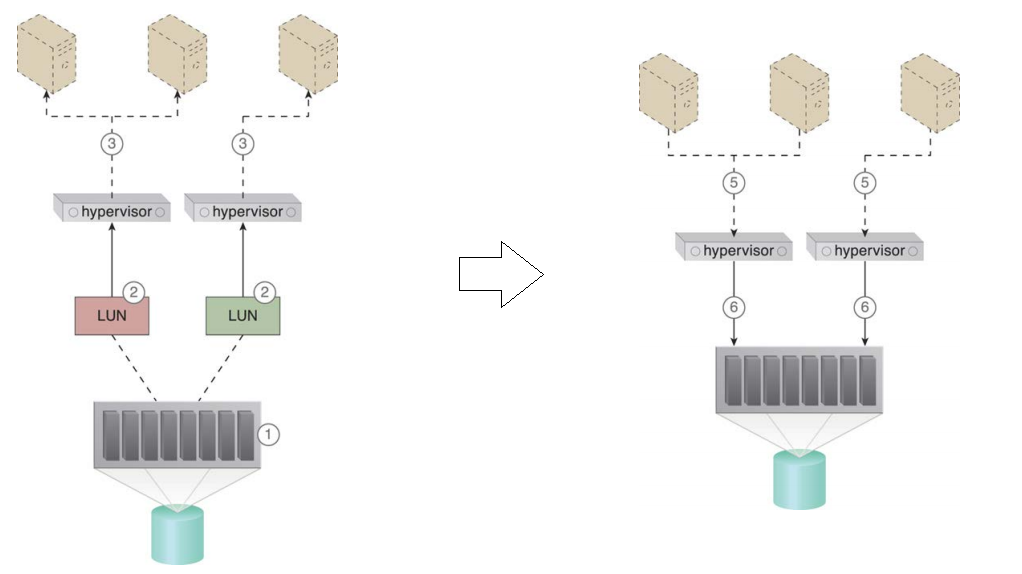
\includegraphics[width=9cm]{./Images/cap13/13.2.png}
\end{figure}

Il cloud storage device viene installato e configurato, dopodiché vengono impostati gli hypervisor in modo che possano avere accesso alle LUN, e mostrano lo storage a cui possono accedere ai virtual server sovrastanti. Lo storage appare come se fosse uno storage normale, ma invece è emulato. La soluzione è di fare in modo di presentare direttamente le LUN ai server virtuali, in modo che questi possano accedere direttamente ai volumi e non ad un "servizio" che mostra lo storage come file-based.

I meccanismi utilizzati sono:
\begin{itemize}
    \item Virtual server
    \item Hypervisor
    \item Cloud storage device
    \item Cloud usage monitor, per avere informazioni sull'utilizzo diretto delle LUN.
    \item Pay-Per-Use Monitor: raccoglie informazioni sull'utilizzo per decidere i costi.
    \item Resource Replication, per sostituire file-based storage con block-based storage.
\end{itemize}

\subsection{Dynamic Data Normalization}
La ridondanza dei dati può causare una serie di problemi negli ambienti cloud, ad esempio l'aumento del tempo necessario a salvare e catalogare i file, l'aumento dello storage necessario per il backup e l'aumento dei costi dovuto a capacità di archiviazione più elevate. Se un consumer carica su cloud un file di 100 MB e la ridondanza è di 10 copie, il consumer pagherà e avrà bisogno di 1000 MB, senza contare il fatto che sarà necessario più tempo per recuperare ed archiviare il file. 

La Dynamic Data Normalization Architecture stabilisce un sistema di "de-duplicazione", che impedisce al cloud consumer di sprecare più risorse di quante ne siano veramente necessarie per quanto riguarda la ridondanza dei dati. Questo sistema può essere applicato sia al block-based storage che al file-based, ma è più efficiente sul primo. Di ogni blocco viene calcolato l'hash e viene controllato per determinare se è stato già ricevuto o meno. I blocchi ridondanti vengono sostituiti da puntatori all'effettivo blocco che è archiviato.

\begin{figure}[htb!]
    \centering
    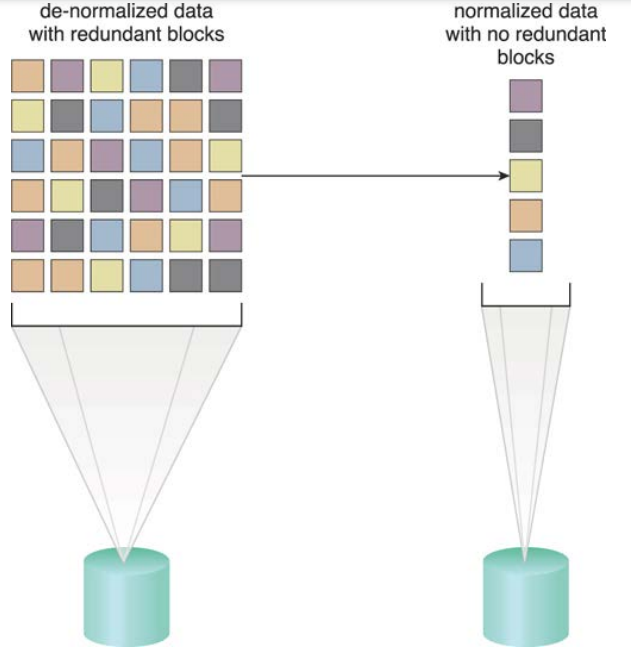
\includegraphics[width=8cm]{./Images/cap13/13.3.png}
\end{figure}

\subsection{Device Vertical Tiering}
Il Device Vertical Tiering è un'architettura che permette di rendere le risorse scalabili anche in particolari situazioni dove potrebbe apparire difficile effettuare uno scaling a causa di restrizioni denotate dall'hardware. Distinguiamo due tipi di DVT: intra-storage e cross-storage.

\subsubsection{Intra-storage DVT}
Alcuni cloud consumer potrebbero avere dei requisiti di data storage restrittivi che obbligano le risorse ad essere archiviate su un singolo Cloud Storage Device, magari a causa della sicurezza dei dati, della privacy, o per motivi legislativi. Il Device Vertical Tiering intra-storage stabilisce un sistema che supporta lo scaling verticale in un singolo cloud storage device: per implementare questo meccanismo è necessario l'utilizzo di uno storage complesso che supporti diversi tipi di dischi, specialmente quelli ad alte prestazioni. I tipi di dischi sono poi organizzati in livelli in modo che le LUN possano migrare verticalmente tra i dischi di livelli diversi.

\begin{figure}[htb!]
    \centering
    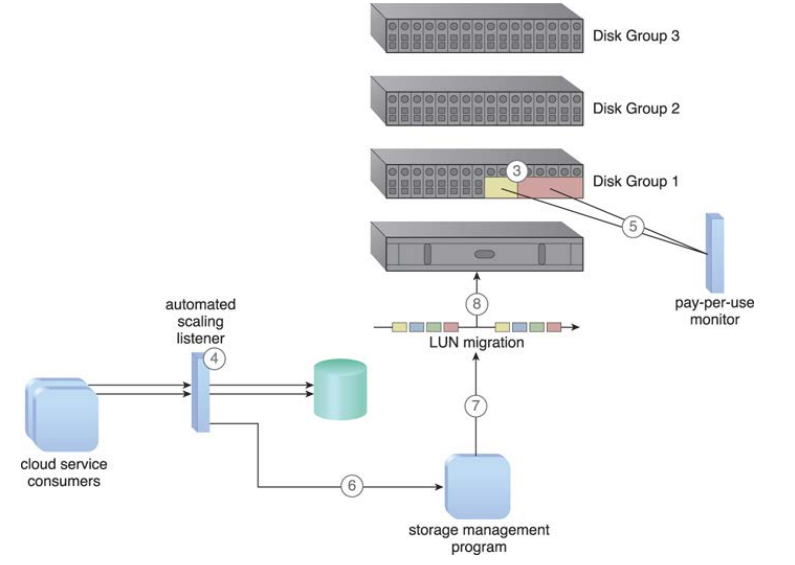
\includegraphics[width=9cm]{./Images/cap13/13.4.png}
\end{figure}

Nella figura sono state create due LUN sul Disk Group 1 (3). L'Automated Scaling Listener monitora le richieste in relazione a soglie predefinite (4). Il Pay-Per-Use Monitor traccia l'ammontare attuale di disco utilizzato (5). L'ASL determina che il numero di richieste sta raggiungendo una soglia e informa lo storage management program che le LUN devono essere spostate su un Disk Group più performante (6). Viene quindi avviato il programma di migrazione LUN (7) e le LUN vengono spostate (8).

\subsubsection{Cross-storage DVT}
I tradizionali metodi di scaling verticale possono risultare inefficienti o time-consuming quando oltre ad aumentare la quantità di richieste aumentano di colpo le specifiche di potenza, storage e rete richieste. Il Device Vertical Scaling cross-storage stabilisce un sistema che riesce a sopperire ai limiti dettati dalla potenza e dalla larghezza di banda scalando tra device che hanno capacità differenti. Le LUN possono fare scaling up e down automaticamente tra diversi device in questo sistema in modo che le richieste utilizzano il device più consono al loro livello di requisiti. L'ASL monitora le richieste inviate alle singole LUN e segnala lo storage management program per spostare un LUN su un altro dispositivo quando viene raggiunta una certa soglia. Il dispositivo originale rimane intatto e le richieste vengono automaticamente smistate al dispositivo più consono.

\begin{figure}[htb!]
    \centering
    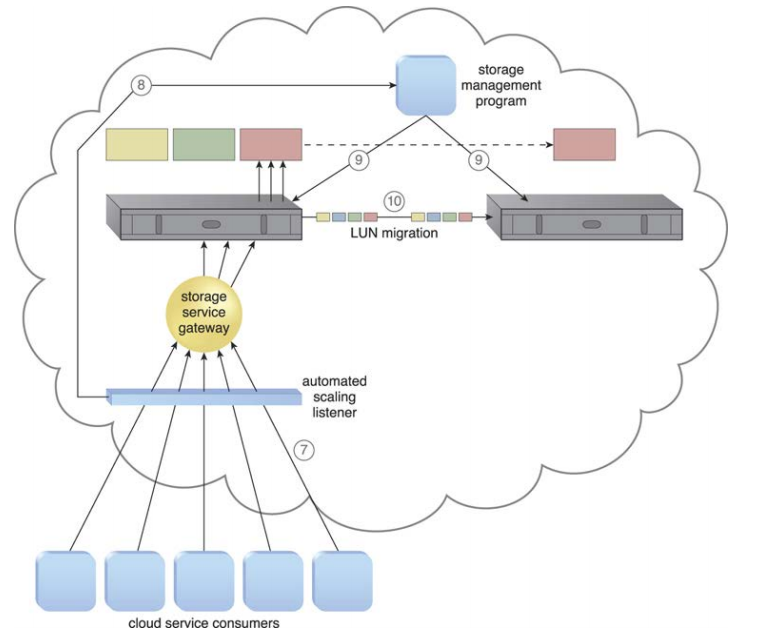
\includegraphics[width=9cm]{./Images/cap13/13.5.png}
\end{figure}

I meccanismi utilizzati sono: 
\begin{itemize}
    \item Automated Scaling Listener
    \item Cloud Storage Device
    \item Audit Monitor, controlla che la rilocazione delle risorse rispetti i requisiti legislativi delle regioni in cui si trovano i dispositivi.
    \item Cloud Usage Monitor
    Pay-Per-Use Monitor
\end{itemize}

\subsection{Storage Maintenance Window}
I dispositivi di cloud storage che sono soggetti a manutenzione e task amministrativi a volte necessitano di essere riavviati o spenti, il che implica l'inutilizzabilità delle risorse IT che giacciono al loro interno. Lo Storage Maintenance Window permette ai cloud service consumer di essere redirezionati automaticamente e in modo trasparente verso dispositivi di storage secondari, senza rendere noto che il dispositivo primario è offline, utilizzando un programma di \textbf{Live Storage Migration}\footnote{Un programma di Live Storage Migration è un sistema sofisticato che utilizza le componenti di migrazione delle LUN per spostare le unità logiche in modo \textit{reliable} permettendo alle copie originali di rimanere attive fino a che la copia di destinazione non sia completamente attiva.}

\begin{figure}[htb!]
    \centering
    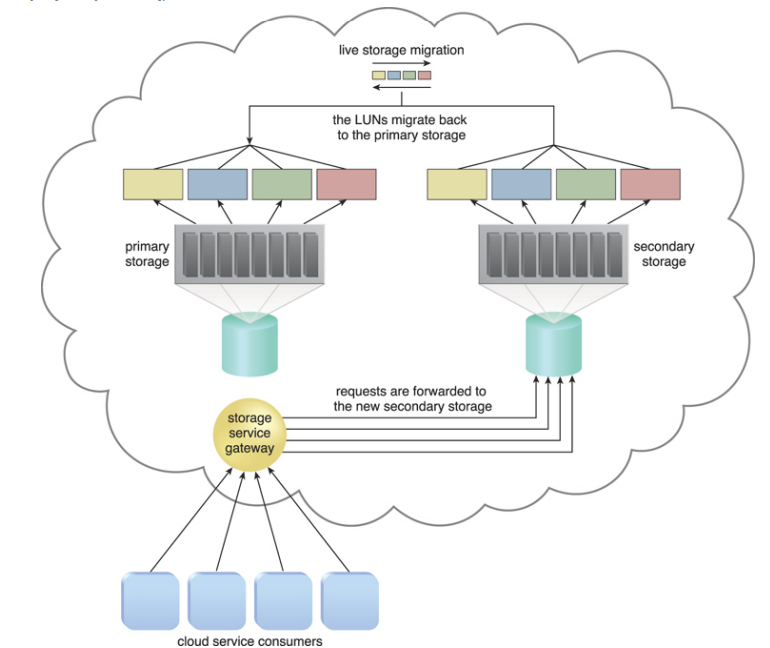
\includegraphics[width=9cm]{./Images/cap13/13.6.png}
\end{figure}

\section{Network related architectures}
\subsection{Elastic Network Capacity}
Nonostante le risorse IT siano distribuite on-demand e in modo scalabile sul cloud, le prestazioni e l'availability possono essere compromesse quando l'accesso remoto alle risorse è colpito da limitazioni alla banda di rete.

Grazie all'elastic network è possibile stabilire un sistema che può allocare larghezza di banda dinamicamente alla rete per evitare colli di bottiglia durante l'esecuzione. Script di intelligent automation engine insieme all'Automated Scaling Listener si occupano di capire quando il traffico raggiunge la soglia stabilita e quindi quando allocare risorse aggiuntive.

\begin{figure}[htb!]
    \centering
    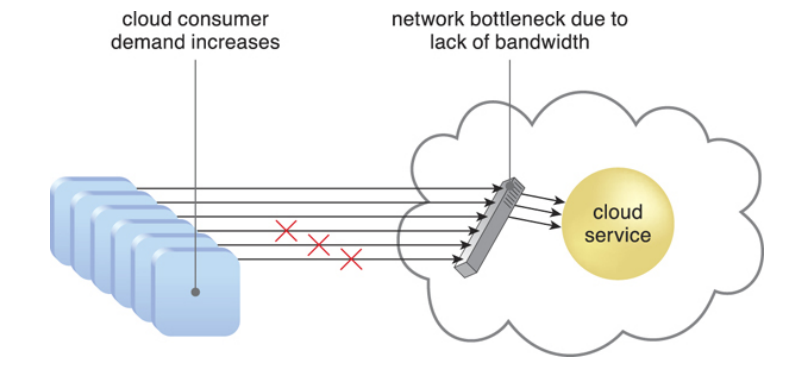
\includegraphics[width=9cm]{./Images/cap13/13.7.png}
\end{figure}

I meccanismi utilizzati sono:
\begin{itemize}
    \item Automated Scaling Listener
    \item Cloud Usage Monitor
    \item Hypervisor
    \item Logical Network Perimeter
    \item Pay-Per-Use Monitor
    \item Resource Replication, per aggiungere server e porte
    \item Virtual Server
\end{itemize}

\subsection{Load Balanced Virtual Switches}
I server virtuali sono collegati al mondo esterno tramite dei virtual switch, che inviano e ricevono dati. Ovviamente possono verificarsi rallentamenti dovuti a problemi di prestazioni, perdita di pacchetti, o lag time. L'architettura di Load Balanced Virtual Switches permette di bilanciare il carico tramite diversi uplink che distribuiscono il traffico di dati attraverso diversi path ridondanti, per evitare trasferimenti lenti di dati.

\begin{figure}[htb!]
    \centering
    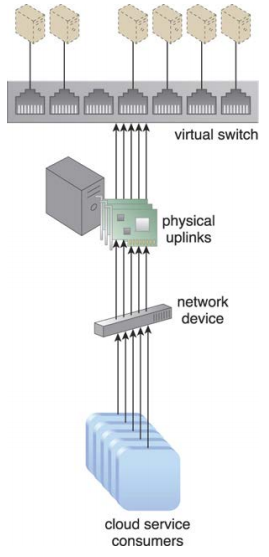
\includegraphics[width=5cm]{./Images/cap13/13.8.png}
\end{figure}

I virtual switch devono essere configurati per supportare diversi uplink fisici, che normalmente possono gestire diversi flussi di dati.
I meccanismi utilizzati sono:
\begin{itemize}
    \item Cloud Usage Monitor
    \item Hypervisor
    \item Load Balancer
    \item Logical Network Perimeter
    \item Resource Replication
    \item Virtual Server
\end{itemize}

\subsection{Multipath Resource Access}
Alcune risorse IT permettono l'accesso solo attraverso un percorso specifico o un hyperlink che punta alla loro locazione esatta. Questo link potrebbe essere perso dal consumer o cambiato dal provider, rendendo inaccessibile la risorsa e quindi non più disponibile. Il Multipath Resource Access permette di stabilire percorsi alternativi che puntano ad una stessa risorsa, in modo che il cloud consumer vi possa accedere con modalità diverse ed equivalenti. Questa architettura richiede l'utilizzo di un multipathing system e la creazione di hyperlink virtuali o fisici che siano assegnati alle risorse. Il multipathing system risiede sul server o su un hypervisor e controlla che ogni risorsa sia accessibile in modo equivalente da tutti i suoi hyperlink.

\begin{figure}[htb!]
    \centering
    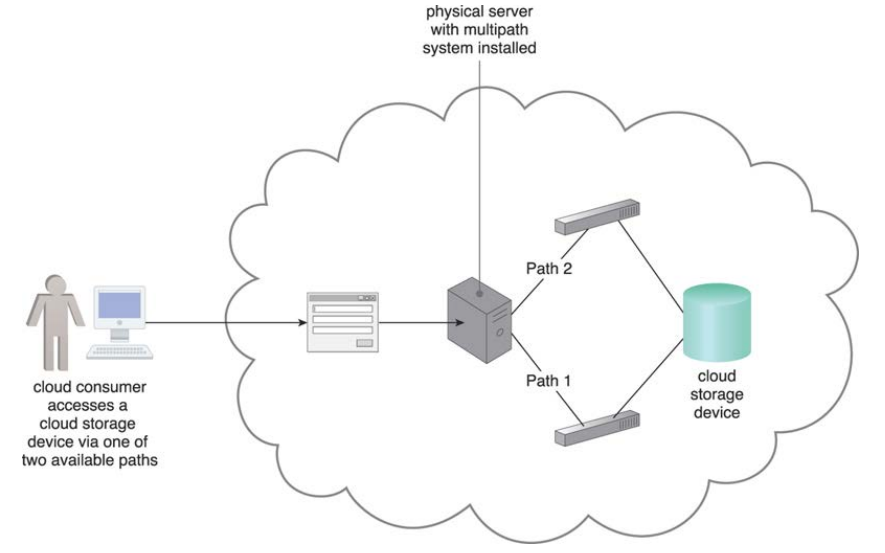
\includegraphics[width=9cm]{./Images/cap13/13.9.png}
\end{figure}

I meccanismi utilizzati sono:
\begin{itemize}
    \item Cloud Storage Device
    \item Hypervisor
    \item Logical Network Perimeter, che garantisce la privacy del cloud consumer anche quando vengono creati percorsi aggiuntivi per una risorsa.
    \item Resource Replication
    \item Virtual Server
\end{itemize}

\subsection{Persistent Virtual Network Configuration}
La configurazione di rete e l'assegnamento delle porte per i virtual server viene generata durante la creazione dei virtual switch sul server fisico ospitante e sull'hypervisor. Queste configurazioni sono salvate nell'ambiente di hosting del virtual server, per cui se questo viene rilocato su un altro server fisico si verificano quasi sicuramente problemi di connessione dovuti alla non configurazione delle porte e delle informazioni di rete. Grazie alla Persistent Virtual Network Configuration, le informazioni di connessione sono salvate in una locazione centralizzata e replicate sui server fisici che fungono da host. In questo modo è possibile migrare un server virtuale verso un altro server fisico senza che ci sia la necessità di effettuare un'ulteriore configurazione.

\begin{figure}[htb!]
    \centering
    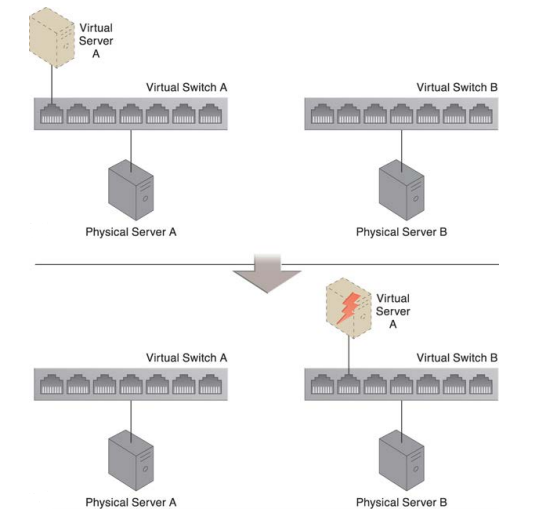
\includegraphics[width=9cm]{./Images/cap13/13.10.png}
\end{figure}

I meccanismi utilizzati sono:
\begin{itemize}
    \item Virtual server
    \item Hypervisor
    \item Logical Network Perimeter
    \item Resource Replication
\end{itemize}

\subsection{Redundant Physical Connection for Virtual Servers}
Come abbiamo visto in precedenza, un server virtuale si collega al mondo esterno tramite virtual switch collegati ad un uplink. Se l'uplink fallisce, il server diventa isolato e viene disconnesso dal mondo esterno. La Redundant Physical Connection for Virtual Servers permette di configurare più connessioni per diversi uplink e impostarne alcune in standby. In questo modo si crea un'architettura ridondante di uplink che permette ai server virtual di collegarsi velocemente ad un altro uplink nel caso quello primario fallisca.

\begin{figure}[htb!]
    \centering
    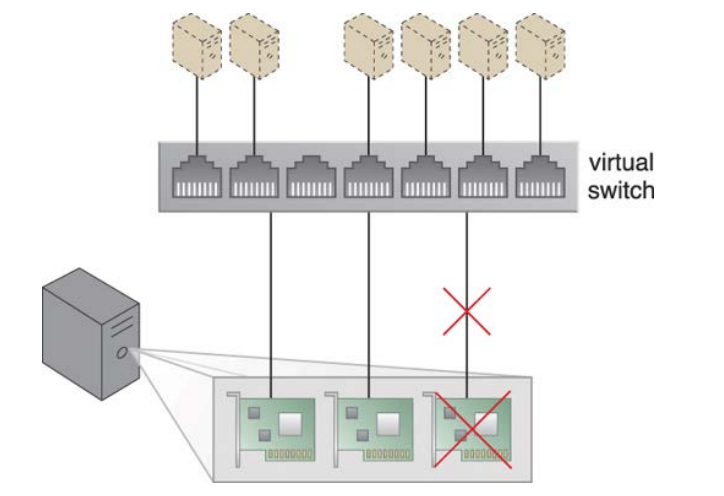
\includegraphics[width=9cm]{./Images/cap13/13.11.png}
\end{figure}

I meccanismi utilizzati sono:
\begin{itemize}
    \item Virtual Server
    \item Hypervisor
    \item Logical Network Perimeter, per assicurare che le connessioni ad un uplink di un consumer rimangano isolate dagli altri.
    \item Resource Replication
\end{itemize}

\section{Learning Check}
\begin{enumerate}
    \item Descrivi l'obiettivo dell'architettura Direct I/O Access e spiega come fa sì che sia possibile l'accesso diretto a una scheda fisica di I/O da parte di un virtual server. Inoltre elenca i meccanismi del Cloud Computing utilizzati in questa architettura.
    \item Descrivi gli obiettivi dell'architettura Direct LUN Access e spiega come grazie ad essa è possibile che un virtual server acceda allo storage block-based delle LUN. Inoltre elenca i meccanismi del Cloud Computing utilizzati in questa architettura.
    \item Descrivi l'obiettivo dell'architettura Dynamic Data Normalization e spiega cos'è la de-duplicazione e come fa ad evitare l'archiviazione di dati ridondanti. Inoltre elenca i meccanismi del Cloud Computing utilizzati in questa architettura.
    \item Descrivi l'obiettivo dell'architettura Elastic Network Capacity e descrivi l'utilizzo dell'Automated Scaling Listener e degli script automatici. Inoltre elenca i meccanismi del Cloud Computing utilizzati in questa architettura.
    \item Descrivi l'obiettivo dell'architettura Cross-Storage Device Vertical Tiering e spiega come realizza il vertical tiering con dispositivi di cloud storage con capacità differenti. Inoltre elenca i meccanismi del Cloud Computing utilizzati in questa architettura.
    \item Descrivi l'obiettivo dell'architettura Intra-Storage Device Vertical Tiering e spiega l'utilizzo relativo di diversi tipi di dischi. Inoltre elenca i meccanismi del Cloud Computing utilizzati in questa architettura.
    \item Descrivi l'obiettivo dell'architettura Load Balanced Virtual Switches e spiega come fa a fornisre uplink multipli per scopi di bilanciamento del traffico di rete. Inoltre elenca i meccanismi del Cloud Computing utilizzati in questa architettura.
    \item Descrivi l'obiettivo dell'architettura Multipath Resource Access e spiega come il suo sistema di multipathing viene utilizzato per fornisre percorsi di accesso alternativi alle risorse. Inoltre elenca i meccanismi del Cloud Computing utilizzati in questa architettura.
    \item Descrivi l'obiettivo dell'architettura Persistent Virtual Network Configuration e spiega l'utilizzo della VIM e di un virtual switch centralizzato per archiviare e rendere disponibili le configurazioni di rete dei virtual server. Inoltre elenca i meccanismi del Cloud Computing utilizzati in questa architettura.
    \item Descrivi l'obiettivo dell'architettura Redundant Physical Connection for Virtual Servers e spiega perché utilizza connessioni di rete a backup fisici. Inoltre elenca i meccanismi del Cloud Computing utilizzati in questa architettura.
    \item Descrivi l'obiettivo dell'architettura Storage Maintenance Window e spiega il suo utilizzo del meccanismo della replicazione di risorse. Inoltre elenca i meccanismi del Cloud Computing utilizzati in questa architettura.
\end{enumerate}
 